\pagebreak
\setauthorname{Lukas Schachinger}
\chapter{Unity}

\section{Einführung}
Unity (auch bekannt als Unity3D) ist eine Game Engine und IDE zum kreieren von Interaktionsmedien, meißt Video Spielen. \Cite[][A history of the unity game engine]{haas2014history} \\ %todo: ide gls %todo: change all citations

Die Game Engine wurde in Kopenhagen in 2005 veröffentlicht und ist bekannt für Spiele wie zum Beispiel: Among Us, Monument Valley, Pokemon Go oder dem Shooter Escape from Tarkov. Die Game Engine wurde mit C++ geschrieben, ermöglicht den Nutzern mittels der zugänglicheren Programmiersprache C\# zu arbeiten. Außerdem bietet die Game Engine die Möglichkeit mit einem Visuellen Editor die Level zu gestalten.

\subsection{Game Objects und Komponenten}
Jedes Game-Object, oder auch Spiel Objekt in Deutsch, kann eine Vielzahl von Komponenten annehmen. Die nächsten Unterkapitel beschreiben verschiedene solcher Komponenten

\subsubsection{Das Mesh}
\glqq A mesh consists of triangles arranged in 3D space to create the impression of a solid object. \grqq \Cite[][Anatomy of a Mesh]{unitydoc}\\
Ein sogenanntes Mesh definiert das physikalische Objekt. Wie in dem Unity Artikel \verb+Anatomy of a Mesh+ beschrieben ist, besteht das Mesh eines Objektes aus, im 3 Dimensionalen Raum positionierten, Dreiecken die ein solides Objekt darstellen sollen.\\
\noindent
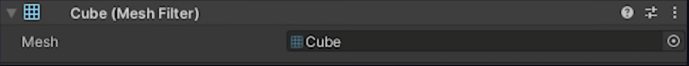
\includegraphics[width=1\linewidth]{chapters/14/Images/Mesh2.png}

\pagebreak

\subsubsection{Der Mesh Renderer}
Der Mesh Renderer ist dafür verantwortlich Materalien und Lichteffekte wie Reflextionen bei einem Objekt darzustellen.\\
\noindent
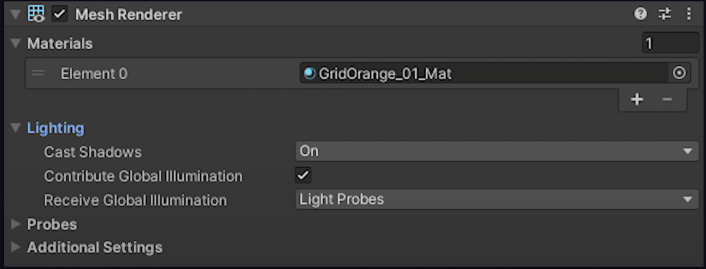
\includegraphics[width=0.7\linewidth]{chapters/14/Images/MeshRenderer.png}

\subsubsection{Die Physics Komponenten}
\glqq Adding a Rigidbody component to an object will put its motion under the control of Unity's physics engine. Even without adding any code, a Rigidbody object will be pulled downward by gravity and will react to collisions with incoming objects if the right Collider component is also present. \grqq \cite[][Rigidbody]{unitydocRigidbody} \\
\noindent
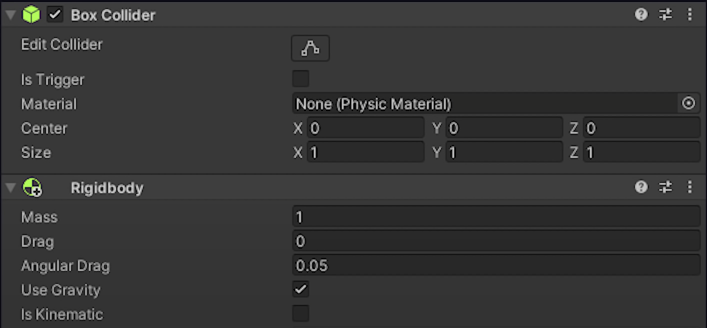
\includegraphics[width=0.7\linewidth]{chapters/14/Images/Physics.png}


\pagebreak
\setauthorname{Martin Usta}
\subsection{Skybox}\
Eine Skybox ist der Hintergrund unsere Spielewelt. Dabei is Skybox ist ein Würfel, indem sich unsere Spielewelt befindet. Die inneren Seiten des Würfels bilden unseren gesamten Hintergrund.
Zu beachten ist das die Würfelseiten die richtige Textur bekommen. Jede Seite hat seine eigene Koordinate für die vergebene Textur:\\\\

\begin{minipage}{0.4\textwidth}
    \begin{itemize}
        \item +Z für vorne 
        \item -Z für hinten 
        \item +X für links 
        \item -X für rechts
        \item +Y für oben
        \item -Y für unten
    \end{itemize}
  \end{minipage}
  \hfill
  \begin{minipage}{0.6\textwidth}
    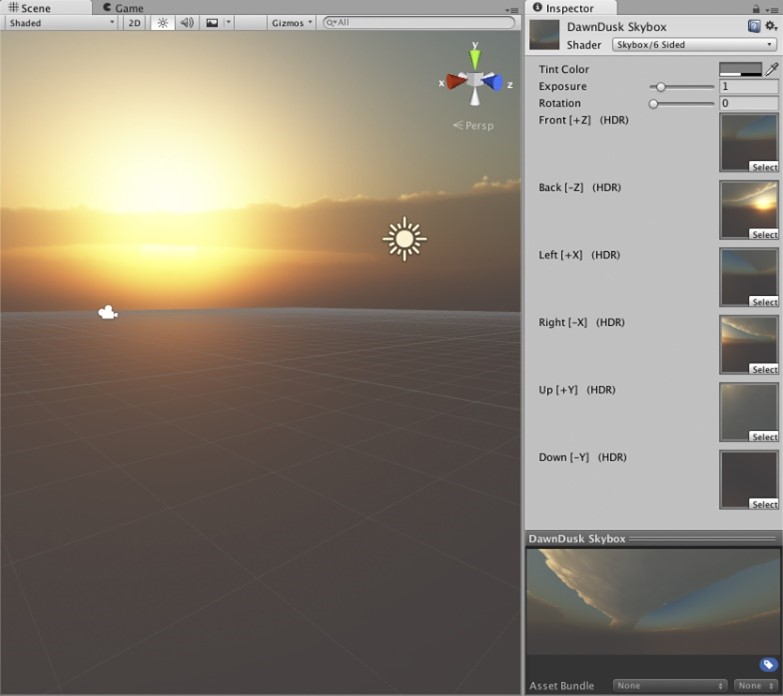
\includegraphics[width=\linewidth]{chapters/14/Images/Skybox.png}
  \end{minipage}